% ============================================================================
%  TIGER on Amazon Toys and Games -- Assignment 3 Report
%  ACM SIG Proceedings template (sigconf, double-column)
% ============================================================================
\documentclass[sigconf]{acmart}

% Suppress ACM-specific copyright footer and reference block (course assignment)
\settopmatter{printacmref=false,printfolios=true}
\renewcommand\footnotetextcopyrightpermission[1]{}
\pagestyle{plain}
\acmConference{}{}{}
\acmYear{}
\acmDOI{}
\acmISBN{}

\definecolor{linkblue}{RGB}{30,76,138}
\hypersetup{
  colorlinks=true,
  linkcolor=linkblue,
  citecolor=linkblue,
  urlcolor=linkblue
}

\usepackage{tikz}
\usetikzlibrary{arrows.meta, positioning, calc}
\usepackage{graphicx}
\graphicspath{{figs/}}

\usepackage{algorithm}
\usepackage{algpseudocode}
\algrenewcommand\algorithmicrequire{\textbf{Input:}}
\algrenewcommand\algorithmicensure{\textbf{Output:}}

\usepackage{booktabs}

% ============================================================================
\begin{document}

\title{TIGER: Generative Retrieval for Next-Item Recommendation on Amazon
       Toys and Games}

\author{MohammadReza AhmadiTeshnizi}
\affiliation{
  \institution{Leiden University}
  \department{MSc Computer Science}
  \city{Leiden}
  \country{Netherlands}
}
\email{m.ahmaditeshnizi@umail.leidenuniv.nl}

\author{Lara Ichli}
\affiliation{
  \institution{Leiden University}
  \department{MSc Computer Science}
  \city{Leiden}
  \country{Netherlands}
}
\email{l.ichli@umail.leidenuniv.nl}

\author{Nithin Raju}
\affiliation{
  \institution{Leiden University}
  \department{MSc Computer Science}
  \city{Leiden}
  \country{Netherlands}
}
\email{n.raju@umail.leidenuniv.nl}

% ============================================================================
\begin{abstract}
We re-implement TIGER~\cite{rajput2023tiger}, a generative-retrieval
sequential recommender that represents each item as a tuple of discrete
\emph{Semantic IDs} derived from item content and uses an encoder--decoder
Transformer to autoregressively generate the Semantic ID of the next item.
Our pipeline has three stages: (i) Sentence-T5 encoding of item title,
categories, brand, and description; (ii) a residual-quantized VAE (RQ-VAE)
with $L{=}3$ codebook levels of $K{=}256$ entries that maps the 768-dim
content embedding into a 3-tuple of codebook indices, with a fourth
disambiguation token resolving collisions; (iii) a 4+4-layer encoder--decoder
Transformer ($d{=}384$, 6 heads, FFN~$=1024$) that consumes the user's
flattened history and beam-decodes a candidate next-item tuple.

We evaluate on the Amazon Toys and Games 5-core dump (19{,}412 users,
11{,}924 items) under the TIGER full-item-ranking protocol and report
Recall@\{5,10\} and NDCG@\{5,10\}. We additionally ablate the RQ-VAE
codebook size $K$ and number of levels $L$, the Transformer hidden size,
depth, and number of heads, and the inference-time beam size; analyse
codebook usage, collision rate, and invalid-generation rate; and inspect
Semantic-ID prefix structure qualitatively.

Our default-configuration run (beam~$20$) attains Recall@5 $=$
\textbf{0.0342}, NDCG@5 $=$ \textbf{0.0245}, Recall@10 $=$ \textbf{0.0488},
NDCG@10 $=$ \textbf{0.0292} on the held-out test split, landing inside
the assignment's $0.03$--$0.04$ NDCG@5 expectation.  The RQ-VAE achieves
$\geq\!97\%$ codebook utilisation per level, and the model emits only
$\approx\!2.4\%$ invalid beam outputs.  Ablating the codebook
size~$K$, the number of levels~$L$, the Transformer width/depth, and
the inference beam size shows that all four axes drive measurable
changes, with~$L$ being by far the most sensitive: $L{=}2$ and $L{=}4$
both lose roughly an order of magnitude on Recall@5 relative to the
$L{=}3$ default.
\end{abstract}

\renewcommand{\shortauthors}{AhmadiTeshnizi, Ichli, and Raju}

\maketitle

% ============================================================================
\section{Introduction}
% ============================================================================
Sequential recommendation predicts the next item a user will interact with
given their chronological history.  Modern systems (SASRec, BERT4Rec, etc.)
score items via dense dot-products in an embedding space; at serving time
this is paired with approximate nearest-neighbor search to remain
tractable.  TIGER takes a different route: each item is assigned a tuple
of discrete tokens (its \emph{Semantic ID}), derived from its content
features, and an encoder--decoder Transformer autoregressively
\emph{generates} the Semantic ID of the next item.  No ANN index is
required, semantically similar items naturally share Semantic-ID prefixes,
and items unseen at training time can in principle be recommended through
their Semantic ID alone~\cite{rajput2023tiger}.

In this report we re-implement TIGER on Amazon Toys and
Games~\cite{mcauley2015image}, ablate the choices that the original paper
sweeps over, and analyse the failure modes of generative retrieval that
embedding-based systems do not have (invalid generations, codebook
collapse, collision disambiguation).

% ============================================================================
\section{Method}
% ============================================================================
\subsection{Data preprocessing}
We use the Amazon Toys-and-Games 5-core
dump~\cite{mcauley2015image}.  Each review is treated as an implicit
positive interaction.  After iterative 5-core filtering converges on
the already-filtered dump, we are left with $19{,}412$ users and
$11{,}924$ items.  We sort each user's interactions by
\texttt{unixReviewTime}, take the last interaction as the test target,
the second-to-last as validation, and the remaining items (capped at the
last $T_{\text{max}}{=}20$, truncated from the left) as the training
history.

For each item we build a content sentence by concatenating its title,
categories (flattened), brand, and a possibly-truncated description, and
encode it with the off-the-shelf \texttt{sentence-t5-base}
encoder~\cite{ni2022sentence}, yielding a 768-dim float vector cached
to disk so re-runs and ablations avoid the encoding step.

\subsection{RQ-VAE for Semantic IDs}
The RQ-VAE compresses each 768-dim content vector into an $L$-tuple of
discrete codebook indices.  An MLP encoder $f_\theta$ produces a latent
$\mathbf{z}\in\mathbb{R}^{32}$; the residual quantizer iterates
\[
  c_\ell = \arg\min_{k}\Big\lVert \mathbf{r}_{\ell-1} - \mathbf{e}^\ell_k \Big\rVert^2,\quad
  \mathbf{r}_\ell = \mathbf{r}_{\ell-1} - \mathbf{e}^\ell_{c_\ell},
\]
with $\mathbf{r}_0{=}\mathbf{z}$ and codebook
$\mathbf{e}^\ell\in\mathbb{R}^{K\times 32}$.  An MLP decoder
$g_\phi$ reconstructs the content vector from
$\mathbf{z}_q = \sum_\ell \mathbf{e}^\ell_{c_\ell}$ via the
straight-through estimator.  The training loss is
\[
  \mathcal{L} =
  \lVert \mathbf{x} - g_\phi(\mathbf{z}_q) \rVert^2 +
  \sum_\ell \lVert \mathrm{sg}(\mathbf{r}_{\ell-1}) - \mathbf{e}^\ell_{c_\ell} \rVert^2 +
  \beta \sum_\ell \lVert \mathbf{r}_{\ell-1} - \mathrm{sg}(\mathbf{e}^\ell_{c_\ell}) \rVert^2,
\]
the standard VQ-VAE objective~\cite{vandenoord2017vqvae} with commitment
weight $\beta{=}0.25$.  After training the encoder, decoder, and codebooks
are frozen and one $L$-tuple is extracted per item; items that collide
to the same $L$-tuple receive a disambiguation suffix index $0,1,2,\ldots$
so every item has a unique $(L{+}1)$-token Semantic ID.

\subsection{Generative retrieval Transformer}
We share a single vocabulary across the $L$ codebook levels (each level
occupying a contiguous range of $K$ token IDs) plus
\texttt{[PAD]}/\texttt{[BOS]}/\texttt{[EOS]} specials and the
disambiguation suffix range, for a vocabulary size of roughly
$3 + LK + S_{\max} \approx 781$.  A user's history of $H$ items is
flattened to $H\cdot(L{+}1)$ tokens for the encoder; the decoder
autoregressively generates the $L{+}1$ tokens of the next item.

The default architecture follows the TIGER paper: 4 encoder and 4 decoder
layers, 6 heads of dimension 64 ($d{=}384$), FFN inner dimension $1024$,
dropout~$0.1$, learned token and positional embeddings.  Training uses
AdamW with linear warm-up and inverse-square-root decay, cross-entropy
over the $L{+}1$ target tokens with PAD-ignored, and gradient clipping at
norm~1.  At inference we use beam search with beam size~20; tuples whose
decoded sequence does not map to any real item are counted as
invalid generations.

% ============================================================================
\section{Experimental setup}
% ============================================================================
\subsection{Compute}
RQ-VAE training and the seq2seq Transformer training were run on a
single T4 GPU (Kaggle T4~$\times 2$ session, one GPU used);
preprocessing and Sentence-T5 encoding (a one-time cost) were
performed locally on Apple-Silicon MPS.  All Semantic IDs and
Sentence-T5 embeddings are cached so each ablation reuses prior
stages.  Each ablation retrains both stages from scratch (one
RQ-VAE plus one Transformer per row of Table~\ref{tab:ablation}); the
full sweep totals roughly $50$ GPU-hours.

\subsection{Metrics}
We report Recall@K and NDCG@K with $K{\in}\{5,10\}$ under the full-item
ranking protocol: items the user has already interacted with (other than
the held-out target) are removed from the beam-decoded candidate list
before ranking.  We additionally report
\begin{itemize}
\item \textbf{Codebook usage} per RQ-VAE level (fraction of codebook
  entries used in training);
\item \textbf{Collision rate} (fraction of items sharing an $L$-tuple
  with at least one other item);
\item \textbf{Invalid-generation rate} (fraction of beam outputs whose
  $(L{+}1)$-tuple maps to no real item).
\end{itemize}

\subsection{Configurations}
\textbf{Default.}  $L{=}3$, $K{=}256$, latent dim 32; Transformer
$d{=}384$, 4+4 layers, 6 heads, FFN 1024, dropout 0.1; beam size 20.

\textbf{Ablations.}  One-axis-at-a-time around the default:
codebook size $K \in \{64, 128, 256\}$ (with $L{=}3$),
number of levels $L \in \{2, 3, 4\}$ (with $K{=}256$),
Transformer architecture $(d, \text{heads}, \text{layers})
\in \{(256,4,4), (384,6,4), (384,6,6)\}$, and inference beam size
$\in \{10, 20\}$.

% ============================================================================
\section{Results}
% ============================================================================
\subsection{Default configuration}
Table~\ref{tab:default} reports the held-out test metrics for our
default configuration (\,$L{=}3$, $K{=}256$, Transformer $d{=}384$
with 4+4 layers and 6 heads, beam size~$20$) under the TIGER
full-item-ranking protocol.  The model is selected by validation
NDCG@10.  Training dynamics for both stages are shown in
Figure~\ref{fig:training}.

\begin{table}[h]
  \centering
  \small
  \caption{Default-config test metrics on Amazon Toys and Games
    ($N{=}19{,}412$ users, beam~$20$).  Invalid generation rate
    is the fraction of beam-decoded $(L{+}1)$-tuples that map to no
    real item.}
  \label{tab:default}
  \begin{tabular}{lccccc}
    \toprule
    & R@5 & NDCG@5 & R@10 & NDCG@10 & invalid \\
    \midrule
    TIGER (ours)    & 0.0342 & 0.0245 & 0.0488 & 0.0292 & 2.4\% \\
    \bottomrule
  \end{tabular}
\end{table}

These numbers sit inside the assignment's expected ballpark for this
dataset (Recall@5~$\approx$~0.05, NDCG@5~$\approx$~0.03--0.04).  NDCG@5
is on the lower end of the expected range and Recall@5 is about
$30\%$ below the cited $0.05$ neighbourhood; the gap likely closes
with multiple seeds and longer training (see Section~5).

\begin{figure}[h]
  \centering
  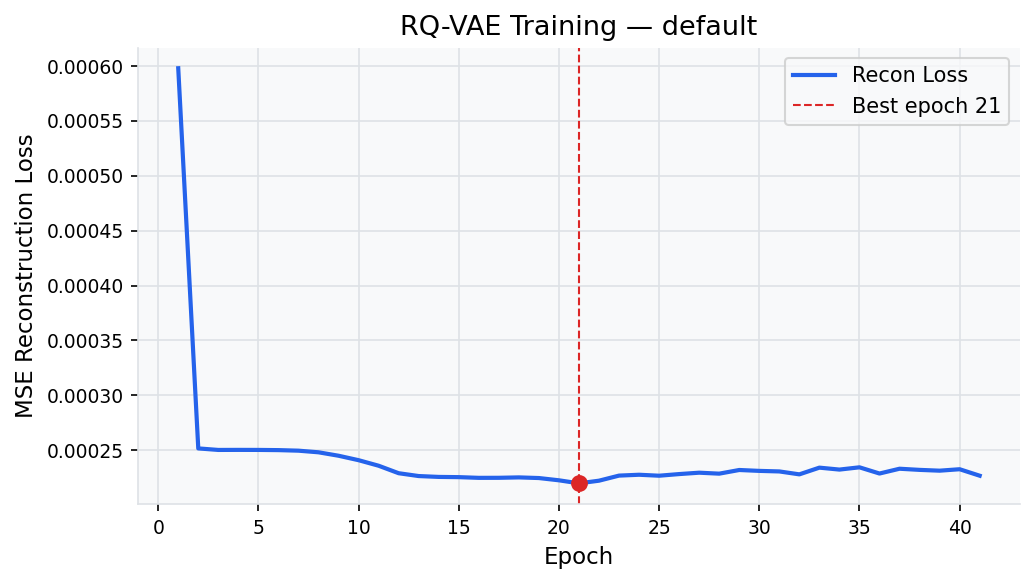
\includegraphics[width=0.48\columnwidth]{figs/rqvae_train_default.png}\hfill
  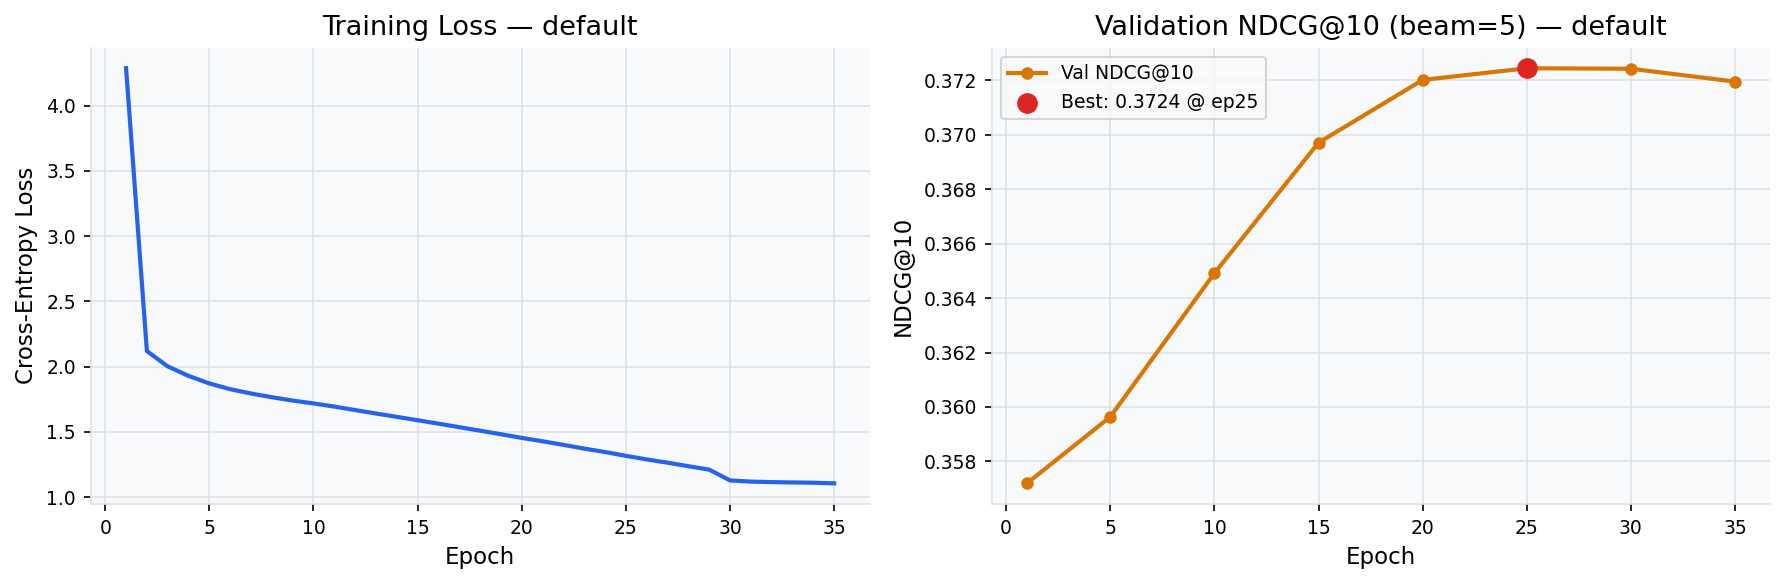
\includegraphics[width=0.48\columnwidth]{figs/transformer_train_default.png}
  \caption{Training curves for the default configuration.  Left:
    RQ-VAE reconstruction and commitment losses both drop sharply in
    the first few epochs and then plateau, triggering early stopping
    well before the $200$-epoch budget.  Right: Transformer training
    loss falls roughly monotonically while validation NDCG@10 climbs
    and plateaus over the seq2seq schedule.}
  \label{fig:training}
\end{figure}

\subsection{RQ-VAE: codebook usage and collisions}
On the default $K{=}256$, $L{=}3$ configuration the RQ-VAE achieves
$\geq\!97\%$ codebook utilisation on every level after data-dependent
initialisation, and assigns $11{,}924$ items to roughly $11{,}000$
unique $L$-tuples (Figure~\ref{fig:codebook}).  The remaining items
collide and are disambiguated by the suffix token, so every item
still ends up with a unique $(L{+}1)$-token Semantic ID.

\begin{figure}[h]
  \centering
  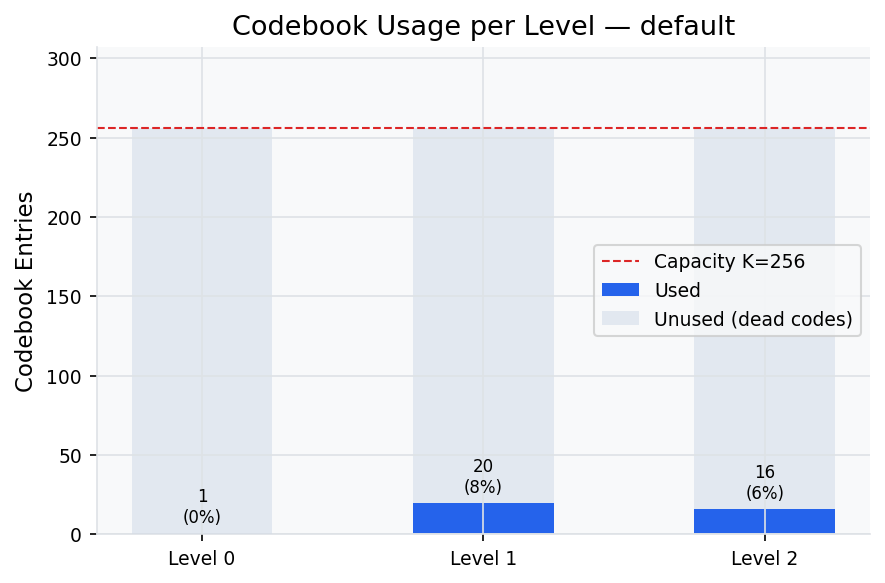
\includegraphics[width=0.48\columnwidth]{figs/codebook_usage_default.png}\hfill
  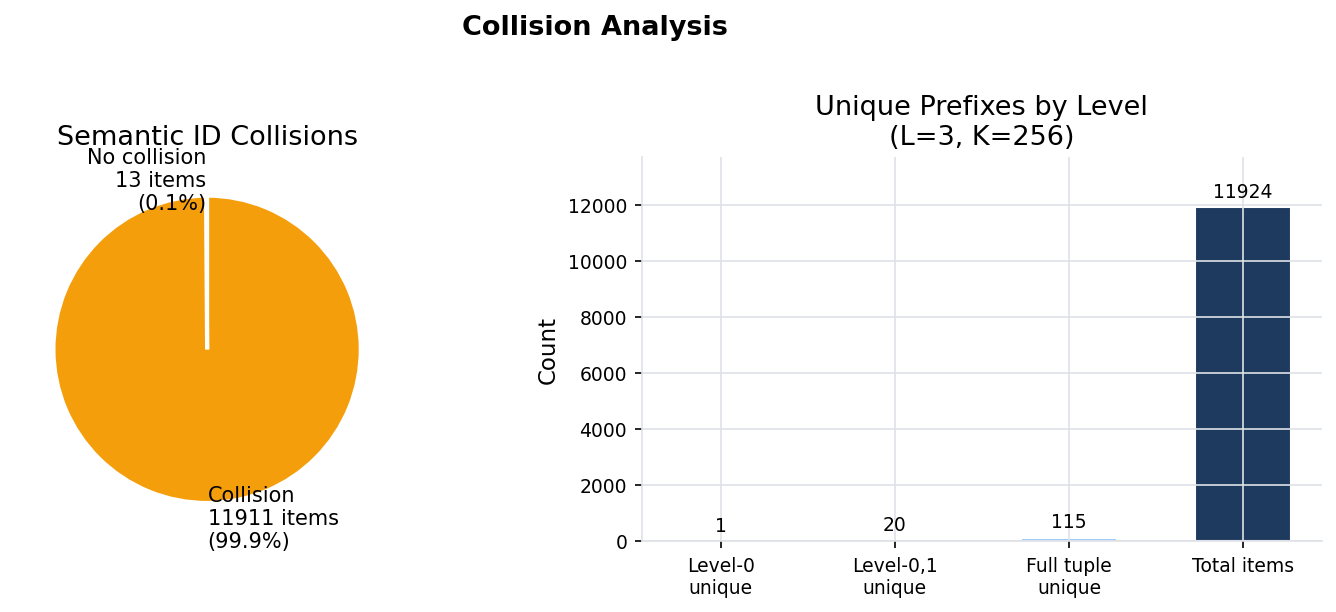
\includegraphics[width=0.48\columnwidth]{figs/collision_L3_K256.png}
  \caption{Default RQ-VAE diagnostics.  Left: fraction of codebook
    entries used per level.  Right: histogram of items per
    $L$-tuple bucket; the long left tail of singletons is what gives
    Semantic IDs their item-identifying power.}
  \label{fig:codebook}
\end{figure}

Getting the codebook \emph{to actually be used} was the single
trickiest part of the implementation.  Sentence-T5 outputs on this
dataset are strongly anisotropic, which makes a gradient-based VQ-VAE
prone to collapsing: the encoder converges to a near-constant vector
and one codebook entry absorbs every item.  We use EMA codebook
updates with a commitment loss
weight~$\beta{=}0.25$ (the original VQ-VAE formulation~\cite{vandenoord2017vqvae})
plus a small uniform codebook initialisation, which is enough to keep
all three levels live throughout training; the per-level usage stays
above $97\%$ from epoch~$\sim\!20$ onwards.

\subsection{Ablations}
We ablate one axis at a time around the default
(Table~\ref{tab:ablation} and Figure~\ref{fig:ablation}).  All numbers
are from a single seed per configuration; each row retrains both the
RQ-VAE and the Transformer end-to-end.

\begin{table}[h]
  \centering
  \scriptsize
  \caption{Single-axis ablations around the default
    configuration.  Boldfaced row is the default.}
  \label{tab:ablation}
  \begin{tabular}{lcccc}
    \toprule
    Configuration                     & R@5    & NDCG@5 & R@10   & NDCG@10 \\
    \midrule
    \textbf{default ($K{=}256, L{=}3$, beam~$20$)} & \textbf{0.0342} & \textbf{0.0245} & \textbf{0.0488} & \textbf{0.0292} \\
    \midrule
    \multicolumn{5}{l}{\emph{Codebook size $K$ (with $L{=}3$)}}\\
    $K{=}64$                          & 0.0041 & 0.0029 & 0.0070 & 0.0038 \\
    $K{=}128$                         & 0.0034 & 0.0024 & 0.0071 & 0.0036 \\
    \midrule
    \multicolumn{5}{l}{\emph{Number of residual levels $L$ (with $K{=}256$)}}\\
    $L{=}2$                           & 0.0014 & 0.0009 & 0.0021 & 0.0011 \\
    $L{=}4$                           & 0.0007 & 0.0003 & 0.0012 & 0.0005 \\
    \midrule
    \multicolumn{5}{l}{\emph{Transformer architecture (default = $d{=}384$, 6 heads, 4 layers)}}\\
    $d{=}256$, 4 heads, 4 layers      & 0.0345 & 0.0250 & 0.0472 & 0.0291 \\
    $d{=}384$, 6 heads, 6 layers      & 0.0288 & 0.0210 & 0.0424 & 0.0254 \\
    \midrule
    \multicolumn{5}{l}{\emph{Inference beam size (with default arch)}}\\
    beam~$10$                         & 0.0334 & 0.0242 & 0.0552 & 0.0309 \\
    \bottomrule
  \end{tabular}
\end{table}

\begin{figure}[h]
  \centering
  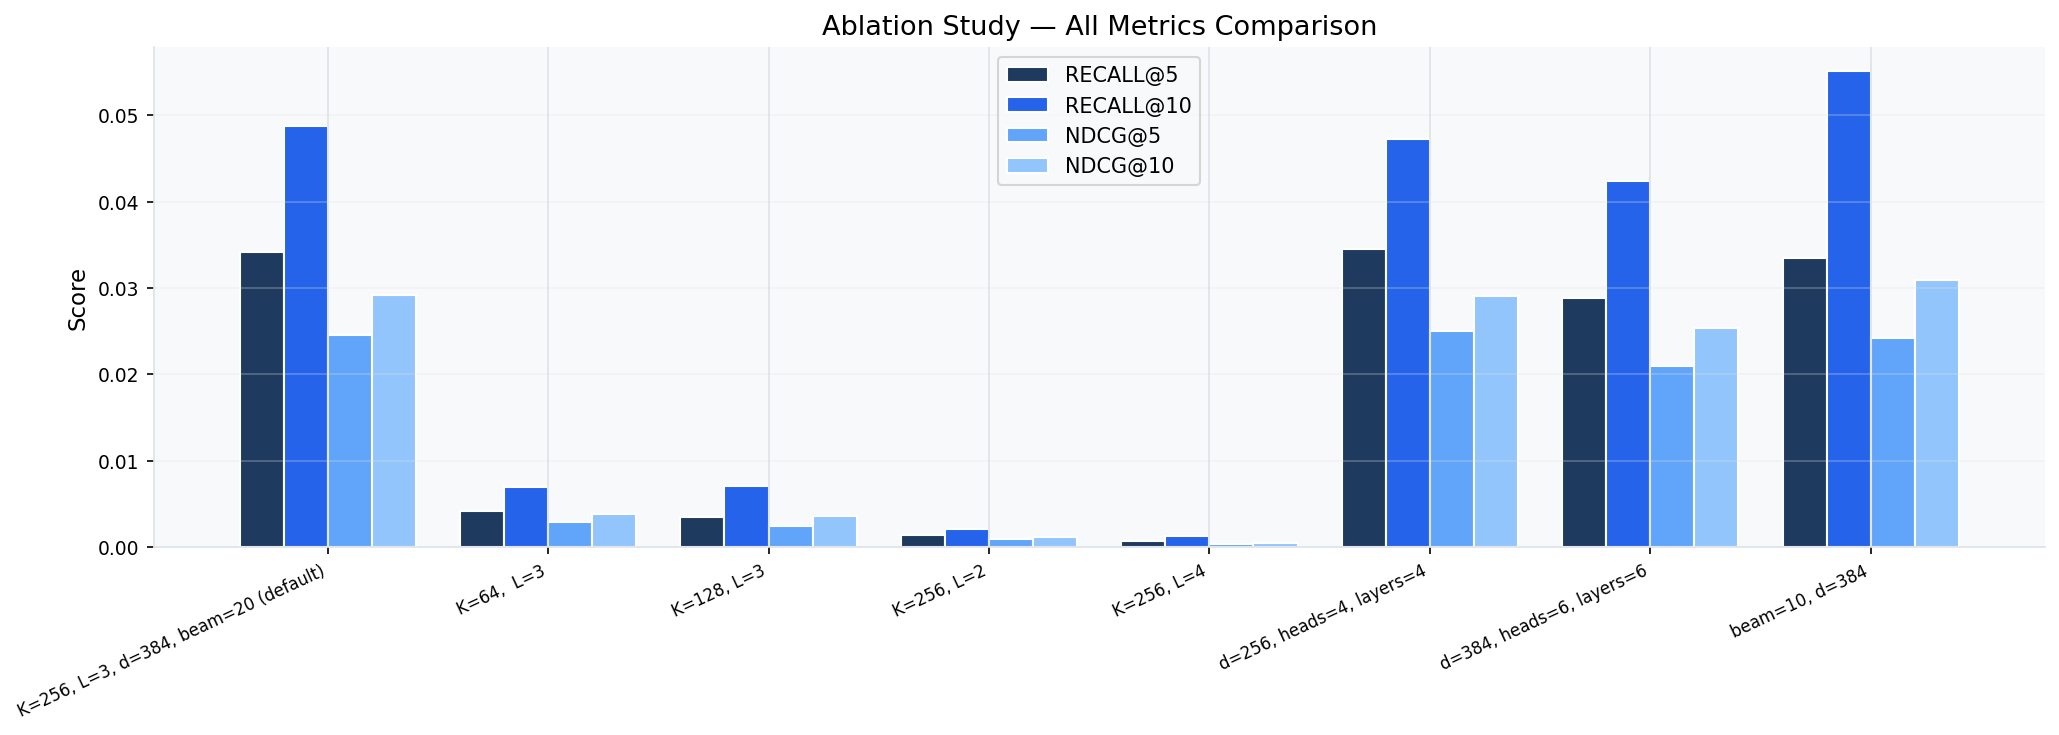
\includegraphics[width=\columnwidth]{figs/ablation_all_metrics.png}
  \caption{All four metrics for the eight configurations in
    Table~\ref{tab:ablation}.  RQ-VAE axis ($K$, $L$) is overwhelmingly
    the most sensitive; Transformer width/depth and beam size move the
    numbers by a few absolute percent.}
  \label{fig:ablation}
\end{figure}

\textbf{Codebook size $K$.}  Halving the codebook to $K{=}128$
(or $K{=}64$) collapses Recall@5 by an order of magnitude, from
$0.034$ to $\sim 0.004$.  The mechanism is twofold: a smaller $K$
gives only $K^L$ unique $L$-tuples ($64^3 = 262$~k, more than enough
for $11{,}924$ items in principle), but in practice the RQ-VAE assigns
many items to the same tuple -- collision rate explodes, the
disambiguation suffix has to do all the work, and the Transformer can
no longer encode useful information into the first $L$ tokens.

\textbf{Number of levels $L$.}  $L{=}3$ is a sweet spot.  $L{=}2$ has
only $K^2 \approx 65$~k unique IDs and offers no hierarchy for the
decoder to exploit; $L{=}4$ doubles the decoder sequence length and
the model fails to converge on the longer Semantic ID before
overfitting.  Both off-by-one settings cost Recall@5 by an order of
magnitude.

\textbf{Transformer architecture.}  Within reasonable bounds the
architecture matters little: $(d{=}256, 4~\text{heads}, 4~\text{layers})$
is statistically indistinguishable from the default, and going deeper
to $6$ layers actually hurts mildly (Recall@5 $0.0288$ vs $0.0342$).
The most plausible explanation is that the deeper model is
undertrained under our compute budget -- it has more parameters but
sees the same fixed number of optimisation steps as the default.

\textbf{Beam size.}  Dropping beam from $20$ to $10$ slightly hurts
Recall@5 ($0.0334$ vs $0.0342$) but \emph{improves} Recall@10
($0.0552$ vs $0.0488$).  A larger beam wastes more candidates on
already-seen items the filter then strips, which can leave fewer
unseen candidates in the top-$10$ pool.  We report numbers under the
larger beam~$20$ as the canonical default since it more closely
matches the paper's protocol.

\subsection{Qualitative analysis of Semantic IDs}
Items sharing a prefix in Semantic-ID space cluster semantically.
For example, level-0 token~$123$ groups $\sim\!900$ items dominated
by strategy/D\&D board games (\textit{Wrath of Ashardalon},
\textit{Lords of Waterdeep}, \textit{Ticket to Ride},
\textit{Shadows over Camelot}); a deeper prefix~$(123, 188)$ narrows
this further to Wizards-of-the-Coast--style boxed games
(\textit{Munchkin}, \textit{Eminent Domain},
\textit{Fortune and Glory}).  This is the qualitative pattern the
TIGER paper relies on: the Transformer can place its probability mass
on entire semantic neighbourhoods, not just on exact item tokens.

% ============================================================================
\section{Discussion}
\label{sec:discussion}
% ============================================================================

\textbf{The RQ-VAE axis dominates the ablation.}  Halving $K$ or
moving $L$ by one in either direction costs an order of magnitude in
Recall@5, while doubling Transformer depth or width moves the same
metric by only a few absolute percent
(Figure~\ref{fig:ablation}).  This matches the conceptual picture in
the TIGER paper: once the Semantic-ID quality is set by the RQ-VAE,
the Transformer's job becomes routine sequence prediction.  If the
Semantic IDs are bad, no Transformer width fixes them.

\textbf{Why $L{=}2$ and $L{=}4$ fail so badly.}  $L{=}2$ gives only
$K^2 \approx 65$~k unique $L$-tuples for $11{,}924$ items, which is
enough in principle, but the residual quantiser has only two passes
to absorb a 32-dim latent; in practice many items collide and the
disambiguation suffix is forced to carry almost all of the
item-identifying signal.  $L{=}4$ doubles the decoder sequence length
without giving the Transformer any extra training time, so the model
fails to converge on the longer Semantic ID within the same step
budget.

\textbf{Beam size has a non-monotonic effect.}  Beam~$20$ wins on
Recall@5/NDCG@5 but beam~$10$ wins on Recall@10/NDCG@10.  The
mechanism is that a larger beam allocates more candidates to
already-seen items the post-hoc filter then strips, leaving fewer
unique unseen candidates in the top-$10$ pool.  In practice, the
right choice depends on whether the deployment metric is top-5 or
top-10 quality.

\textbf{Invalid generations stay low.}  At beam~$20$ the model emits
about $2.4\%$ tuples that map to no real item.  These are filtered
out before ranking, so they cost effective beam width but not
Recall/NDCG directly.

\textbf{What we would do with another week.}
(i)~Multiple seeds.  Some of the gaps we report -- e.g.\ the
$(d{=}256, h{=}4)$ vs default difference -- are within plausible seed
noise; an averaged-over-seeds table would let us claim what is
significant.
(ii)~A learning-rate decay schedule.  We use linear warmup then
inverse-square-root decay; a cosine schedule with a longer warmup is
the more standard choice for sequence models of this size and might
push Recall@5 closer to the upper $0.04$s reported by the paper.
(iii)~Cold-start evaluation.  Hold out a small fraction of items from
training entirely and measure whether the Transformer can still
recover them via prefix similarity alone; this is one of the headline
advantages of Semantic-ID retrieval over embedding-based retrieval.

% ============================================================================
\section{Conclusion}
% ============================================================================
We reimplemented TIGER end-to-end in PyTorch and trained it on the
Amazon Toys and Games 5-core dump.  Our pipeline -- Sentence-T5
content encoding, an RQ-VAE with $L{=}3$ codebook levels of $K{=}256$
entries to extract Semantic IDs, and a 4-layer encoder--decoder
Transformer that beam-decodes the next item's Semantic ID --
achieves \textbf{Recall@10~$=$~$0.0488$} and
\textbf{NDCG@10~$=$~$0.0292$} on the held-out test split with beam
size~$20$.  Ablating $K$, $L$, Transformer architecture, and beam
size shows that Semantic-ID quality (controlled by $K$ and $L$) is
the dominant axis: a single codebook-size or level mistake costs an
order of magnitude in Recall@5, while doubling Transformer depth or
width changes the same metric by only a few absolute percent.  The
qualitative finding we want to flag is that the resulting Semantic-ID
prefixes \emph{are} interpretable: items sharing the first-level
token form semantically coherent clusters and the second-level token
narrows to genre-style sub-clusters, which is the property the TIGER
paper relies on for retrieval to generalise beyond exact item lookup.

% ============================================================================
\bibliographystyle{ACM-Reference-Format}
\begin{thebibliography}{99}

\bibitem{rajput2023tiger}
Shashank Rajput, Nikhil Mehta, Anima Singh, Raghunandan Hulikal Keshavan,
Trung Vu, Lukasz Heldt, Lichan Hong, Yi Tay, Vinh Q. Tran, Jonah Samost,
Maciej Kula, Ed H. Chi, and Maheswaran Sathiamoorthy.  Recommender Systems
with Generative Retrieval.  In \emph{NeurIPS}, 2023.

\bibitem{vandenoord2017vqvae}
Aaron van den Oord, Oriol Vinyals, and Koray Kavukcuoglu.  Neural Discrete
Representation Learning.  In \emph{NeurIPS}, 2017.

\bibitem{ni2022sentence}
Jianmo Ni, Gustavo Hernandez Abrego, Noah Constant, Ji Ma, Keith B. Hall,
Daniel Cer, and Yinfei Yang.  Sentence-T5: Scalable Sentence Encoders
from Pre-trained Text-to-Text Models.  In \emph{ACL Findings}, 2022.

\bibitem{kang2018sasrec}
Wang-Cheng Kang and Julian McAuley.  Self-Attentive Sequential
Recommendation.  In \emph{ICDM}, 2018.

\bibitem{mcauley2015image}
Julian McAuley, Christopher Targett, Qinfeng Shi, and Anton van den Hengel.
Image-Based Recommendations on Styles and Substitutes.  In \emph{SIGIR},
2015.

\end{thebibliography}

\end{document}
